\documentclass[a4paper, 11pt]{article}
\usepackage{geometry}
\usepackage{graphicx}
\usepackage{mathspec} % includes fontspec
\usepackage[natbibapa]{apacite}
\usepackage[font={small,sf}]{caption}

\geometry{a4paper,total={150mm,237mm},inner=30mm,top=30mm}
\defaultfontfeatures{Mapping=tex-text,Scale=MatchLowercase}
\setsansfont{Helvetica}
\setmonofont{Menlo}

\title{Simplicity and informativeness in semantic category systems \\ S1: An introduction to communicative cost}
\author{Jon W. Carr, Kenny Smith, Jennifer Culbertson, Simon Kirby}
\date{}

\begin{document}
\maketitle

\section{Overview}

This document describes Regier and colleagues' information-theoretic model of informativeness, \textit{communicative cost} \citep[see also][]{Regier:2015,Kemp:2018}. The central idea behind communicative cost is that languages may be described as informative to the extent that they minimize the loss of information during interaction. Interaction inherently involves a loss of information because, while the speaker may be certain about the meaning to be expressed, the listener only has access to a word that describes a general category of meanings. There are two main formalizations of communicative cost in the literature, which are adopted according to the particular semantic domain being modeled. We begin by describing the simple discrete case and then move on to the continuous case, which is used in the main paper. Note that some of the notation we use here diverges from the main paper.

\section{The discrete case}

\citet{KempRegier:2012}, who model kinship categories, use the discrete form of communicative cost. Here we give an example where a simple language divides drinking vessels into two categories, cups and mugs. A communicative interaction is illustrated in Fig.~\ref{fg_comm_cost_discrete}. There is a universe of meanings~$U$, and the speaker and listener have a shared language~$L$ that partitions $U$ into categories: $L = \{C_\mathrm{cup}, C_\mathrm{mug}\}$. The speaker wishes to communicate a target meaning~$t \in U$, so she determines which category the target belongs to, for~example $C_\mathrm{mug}$, and transmits its associated word to the listener. The listener maps the word back to the category and selects a meaning~$t^\prime \in C_\mathrm{mug}$. The interaction is considered successful if $t = t^\prime$. In general, the probability that the speaker will successfully communicate some meaning~$m$ using signal~$s$ as an intermediary is~$1/|C_{s(m)}|$; as the cardinality of the category grows, the probability of success decreases because the listener becomes less certain about the speaker's intended meaning \citep[cf.\@ the size principle;][]{Tenenbaum:2001,Xu:2007}. The loss of information, or cost, incurred by using a signal as a proxy for a meaning is therefore $-\log 1 / |C_{s(m)}|$~bits; put differently, the cost is how much additional information the speaker must still send (e.g., additional modifiers) for the listener to pick out the intended meaning.

	\begin{figure}
	\begin{center}
	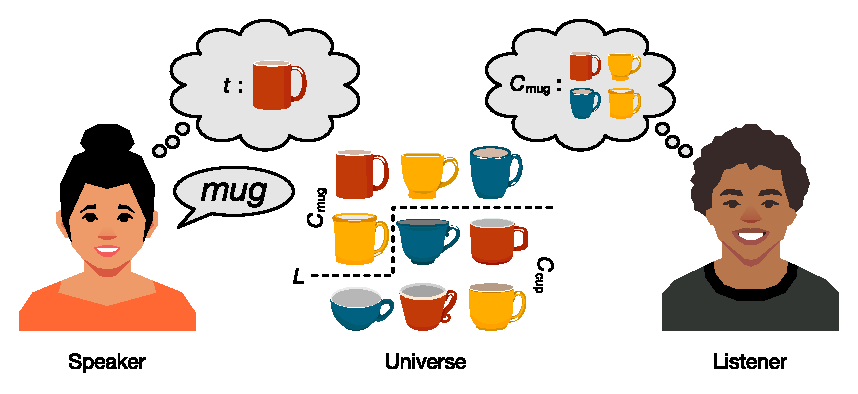
\includegraphics[]{comm_cost_discrete.eps}
	\caption{A speaker wishes to communicate a target meaning~$t$ from a universe of meanings~$U$. She determines which category the target belongs to according to the shared language~$L$, which partitions $U$ into categories, and utters its associated word. The listener maps this word back to a category of possible meanings and must decide on a specific meaning to infer. Here the listener has a $1/4$ chance of correctly inferring the target meaning, since there are four members of the category~$C_\mathrm{mug}$.}
	\label{fg_comm_cost_discrete}
	\end{center}
	\end{figure}

The cost of sending a meaning is modulated by the probability of that meaning occurring $p(m)$, which Regier and colleagues refer to as the ``need probability.'' Thus, the expected cost of a language as a whole is given by

	\begin{equation}
	\mathrm{cost}(L) = \sum_{m \in U} p(m) \cdot -\log 1 / |C_{\mathrm{signal}(m)}|
	\label{eq_cost_discrete}
	\end{equation}

\noindent
For each meaning in the universe, we multiply the probability of that meaning occurring by how much information is lost when a category/signal is used as a proxy for that meaning. This definition of communicative cost has a natural interpretation in information theory: It is the expected number of additional bits required to unambiguously encode a meaning beyond the number of bits transmitted. If the universe consists of 64 equally probable meanings, such that a lossless codeword would require $\log 64 = 6$~bits, but the interlocutors use a system of four equally sized categories, such that a lossy codeword would require $\log 4 = 2$~bits, the communicative cost is $6 - 2 = 4$~bits.

%%%%%%%%%%%%%%%%%%%%%%%%%%%%%%%%%%%%%%%%%%%%%%%%%%%%%%%%%%%%%%%%%%%%%%%%%%%%%%%%%%%%%%%%%%%%

\section{The continuous case}

The definition of communicative cost above assumes that, on hearing a word, the listener is equally likely to infer each member of the associated category. As such, it is only sensitive to expressivity---how many categories are available---and the extent to which category sizes reflect the need probabilities. While this may be appropriate in cases where categories are discrete (e.g., Kemp and Regier's \citeyearpar{KempRegier:2012} study of kinship terms), it is overly-simplistic in others because it fails to model two well-known effects of human categorization: Categories may have fuzzy boundaries, and some category members may be more prototypical than others \citep{Rosch:1973}. Therefore, in work with continuous meanings \citep[such as the color term study in][]{Regier:2015}, the following extended notion of communicative cost is used, in which the probability of a successful interaction is not simply $1/|C|$ but a value related to the distance between intended and inferred meanings. An example of this is illustrated in Fig.~\ref{fg_comm_cost_continuous}.

	\begin{figure}
	\begin{center}
	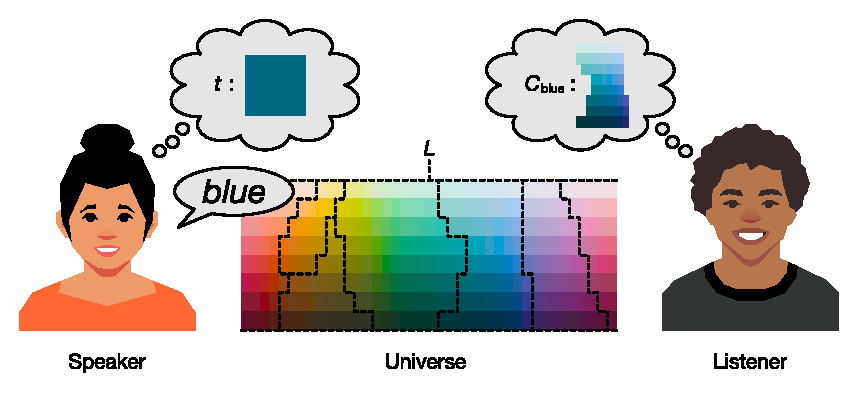
\includegraphics[]{comm_cost_continuous.eps}
	\caption{A speaker wishes to communicate a target meaning~$t$ from a universe of meanings. She determines which category the target belongs to according to the shared language~$L$, which partitions the universe into categories, and utters its associated word. The listener maps this word back to a category of possible meanings and must decide on a specific meaning to infer. He is more likely to infer prototypical (central) members of the category.}
	\label{fg_comm_cost_continuous}
	\end{center}
	\end{figure}

Rather than treat each category~$C$ as a \textit{set} of meanings, each category will now be treated as a probability distribution over all~$m \in U$. To transform a set~$C$ into a distribution~$\tilde{C}$, we assume that the probability of inferring a meaning is proportional to its total similarity to all category members~$m^\prime \in C$:

	\begin{equation}
	\tilde{C}(m) \propto \sum_{m^\prime \in C} \exp -\gamma d(m,m^\prime)^2,
	\label{eq_cost_gaussian}
	\end{equation}

\noindent
where $\gamma > 0$ and $d(\cdot,\cdot)$ gives the distance between two meanings. The term $\exp -\gamma d(m,m^\prime)^2$ relates distance to perceived similarity: The similarity between a meaning and itself is 1; as the distance between two meanings grows, the similarity approaches 0. The parameter~$\gamma$ controls how quickly similarity decays with distance. The effect of this parameter is illustrated in Fig.~\ref{fg_gaussians}. Essentially, small values model fuzzier category systems in which the boundaries between categories are blurred; as $\gamma$ becomes arbitrarily large, $\tilde{C}(m) = 1/|C|$ if $m \in C$ and 0 otherwise, collapsing to the discrete case described above.

	\begin{figure}
	\begin{center}
	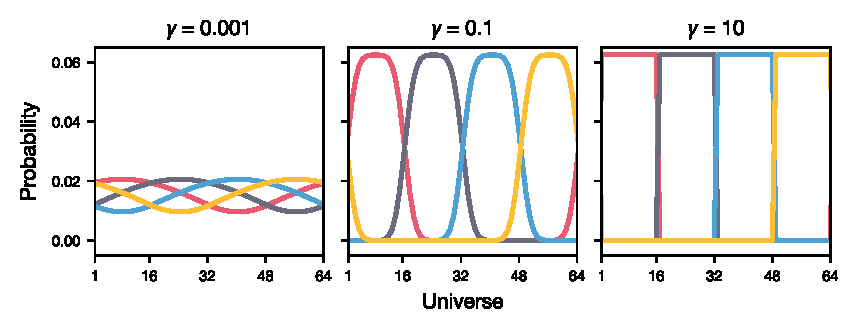
\includegraphics[]{gaussians.eps}
	\caption{A one-dimensional space of 64 meanings is broken up into four equally sized categories. Each probability distribution (indicated in different colors) represents the probability that a listener would infer a given meaning on hearing the word for a given category. The listener is more likely to infer meanings at the center of the category because they are more prototypical. Each plot shows these probability distributions under different settings of $\gamma$. When $\gamma$ is small, category boundaries are very fuzzy; when $\gamma$ is large, the distributions collapse to the discrete case described above.}
	\label{fg_gaussians}
	\end{center}
	\end{figure}

The transformation performed by Equation~\ref{eq_cost_gaussian} models the categories as Gaussians in which the most prototypical meaning (the meaning at the geometric center of the category with the greatest similarity to other category members) has the highest probability of being inferred. Since $\tilde{C}(m)$ gives the probability that the listener will infer meaning~$m$ on hearing the signal for category~$\tilde{C}$, the cost of sending that meaning is~$-\log \tilde{C}(m)$. Therefore, the communicative cost of the language as a whole is given by

	\begin{equation}
	\mathrm{cost}(L) := \sum_{m\in U} p(m) \cdot -\log \tilde{C}_{\mathrm{signal}(m)}(m).
	\label{eq_cost_continuous}
	\end{equation}

\noindent
This is the definition of communicative cost used in the main paper (albeit with a slightly different notation).

\section{Uncertain speakers}

We can now extend what we have so far to cases where the speaker is not entirely certain about the meaning. Indeed, Regier and colleagues usually formulate communicative cost this way. Given a target meaning, the speaker has a distribution $s$, which represents how certain they are about the target meaning. The speaker utters a word according to the category to which the target meaning belongs. On receiving this word, the listener has a distribution $\tilde{C}$, which we will now call the listener distribution $l$. The loss of information is therefore equivalent to the Kullback--Leibler divergence $D_\mathrm{KL}$ between speaker distribution $s$ and listener distribution $l$:

	\begin{equation}
	D_\mathrm{KL}(s||l) = \sum_{m \in U} s(m) \log \frac{s(m)}{l(m)}.
	\label{eq_kullback_leibler}
	\end{equation}

\noindent
Thus, communicative cost may be written as

	\begin{equation}
	\mathrm{cost}(L) := \sum_{m\in U} p(m) D_\mathrm{KL}(s||l).
	\label{eq_cost_kullback}
	\end{equation}

\noindent
This allows for the possibility of modeling speaker uncertainty. Generally, however, speakers are considered to be certain about the target meaning, simplifying the equations to those outlined above.

\section{Properties of informativeness}

According to communicative cost, the extent to which a system may be described as informative is determined by various properties. In the discrete case, the following two properties hold:

	\newcounter{comm_cost_enumeration}
	\begin{enumerate}

		\item \textbf{Expressivity} The more categories a system has, the lower its communicative cost; a system of many categories is informative because the categories pick out smaller, more precise sets of meanings.

		\item \textbf{Balanced cardinality} The more evenly-balanced the category sizes are, the lower the communicative cost of the system as a whole.

		\setcounter{comm_cost_enumeration}{\value{enumi}}
	\end{enumerate}

\noindent
In the continuous case, the following property also applies:

	\begin{enumerate}
		\setcounter{enumi}{\value{comm_cost_enumeration}}
		\item \textbf{Compactness} The more compact categories are, the lower the communicative cost of the system; compact categories are informative because they minimize the distance between intended and inferred meanings.
		\setcounter{comm_cost_enumeration}{\value{enumi}}
	\end{enumerate}

\noindent
Finally, if the need probabilities are nonuniform, properties two and three above may be overridden in favor of smaller categories for frequent meanings and larger categories for infrequent meanings \citep[see e.g.,][]{Regier:2016,Gibson:2017}. This leads to a fourth property of informativeness:

	\begin{enumerate}
		\setcounter{enumi}{\value{comm_cost_enumeration}}
		\item \textbf{Reflection of need} When categories reflect the needs of the interlocutors, the communicative cost of the system is lowered.
	\end{enumerate}

%%%%%%%%%%%%%%%%%%%%%%%%%%%%%%%%%%%%%%%%%%%%%%%%%%%%%%%%%%%%%%%%%%%%%%%%%%%%%%%%%%%%%%%%%%%%
\bibliographystyle{apacite}
\bibliography{/Users/jon/master.bib}
%%%%%%%%%%%%%%%%%%%%%%%%%%%%%%%%%%%%%%%%%%%%%%%%%%%%%%%%%%%%%%%%%%%%%%%%%%%%%%%%%%%%%%%%%%%%

\end{document}